\documentclass[12pt]{article}

\usepackage{graphicx}
\usepackage{fullpage}

\title{TI2200 Practical report\\
Assignment 2 (AIS-E)}
\author{Michiel Haisma 1512285\\
Joost Meulenbeld \\
Boy Bos\\
Leon Loopik 4097718\\
TU Delft\\}
\date{\today}


\begin{document}

\maketitle

\section*{Assignment 1}
To get an idea of the architectural design, a class diagram of the program is created. Using a class diagram, it is possible to quickly see the relations between classes and their attributes and methods. When trying to add features to the system, one should first figure out where the new code should be implemented and what possible effects this could have on other classes. A class diagram gives this information.

The systems basic overview can be seen in figure \ref{lib_total_overview}. Here we devided the system into four modules: the Service module, the Domain module, the GIS module and the Utility module. Each of these modules, except for the Utility module, consist of multiple lower level modules and classes. Therefore, everyone of these modules have a personal class diagram, which can be found in \ref{lib_domain_total}, \ref{lib_service_total} and \ref{lib_gis_total}.

\begin{figure}
  \centering
  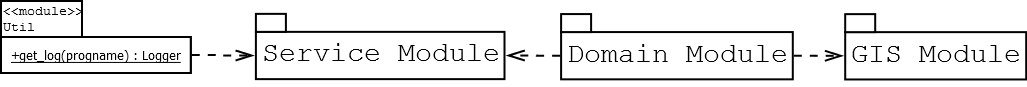
\includegraphics[width=4in]{lib_total_overview}
  \caption{An overview of the interaction between the four basic modules, which build the system.}
  \label{lib_total_overview}
\end{figure}

\begin{figure}
  \centering
  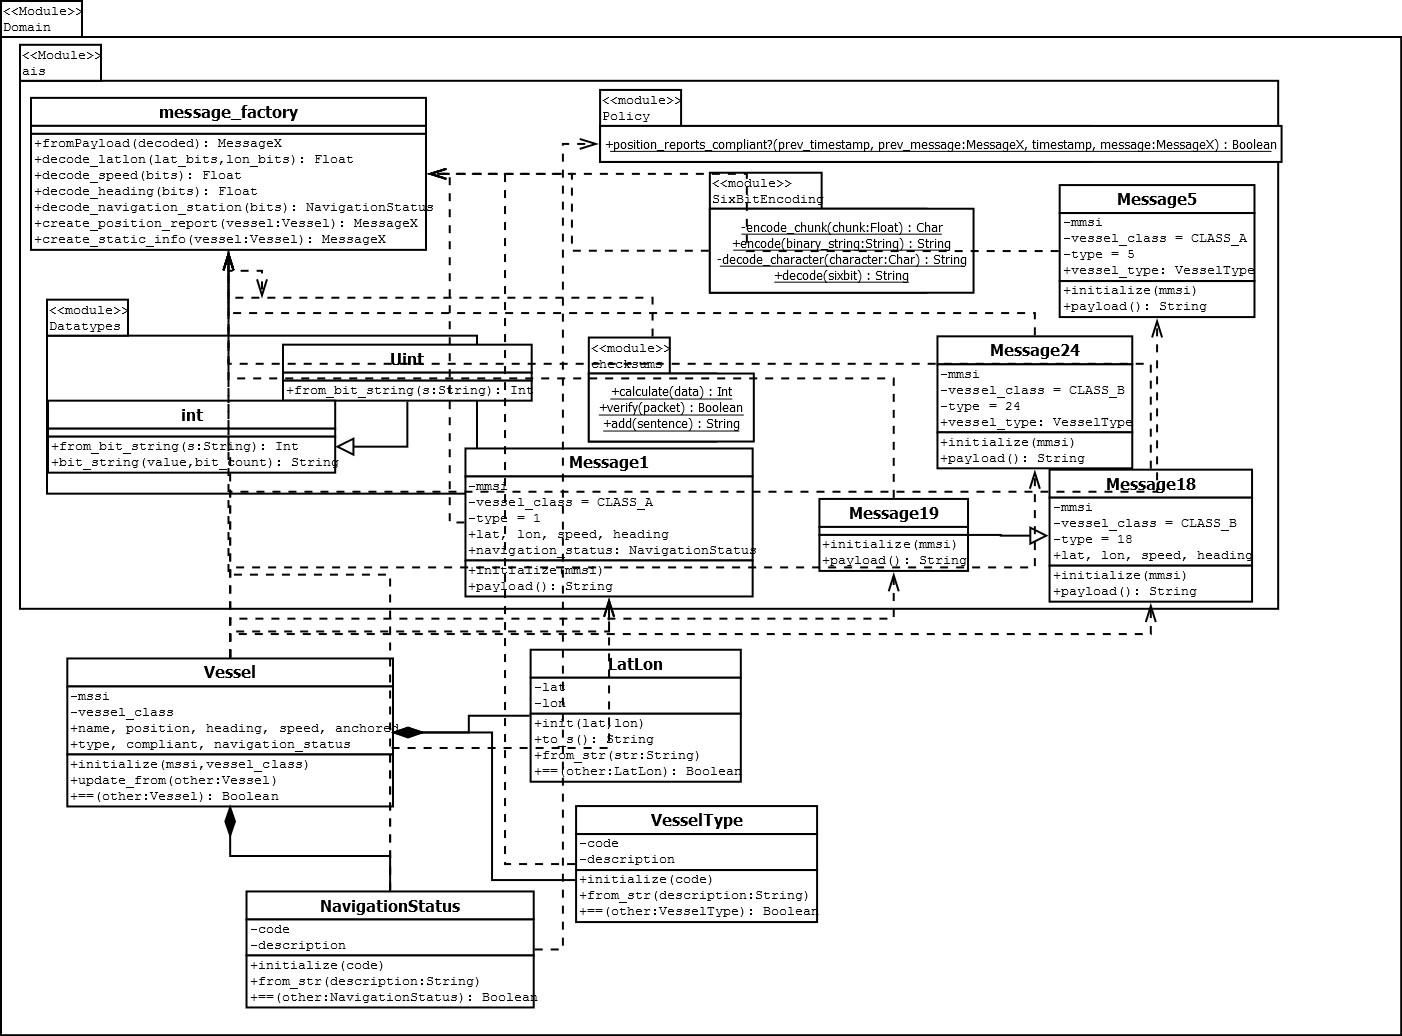
\includegraphics[width=5in]{lib_domain_total}
  \caption{A class diagram of the Domain module.}
  \label{lib_domain_total}
\end{figure}

\begin{figure}
  \centering
  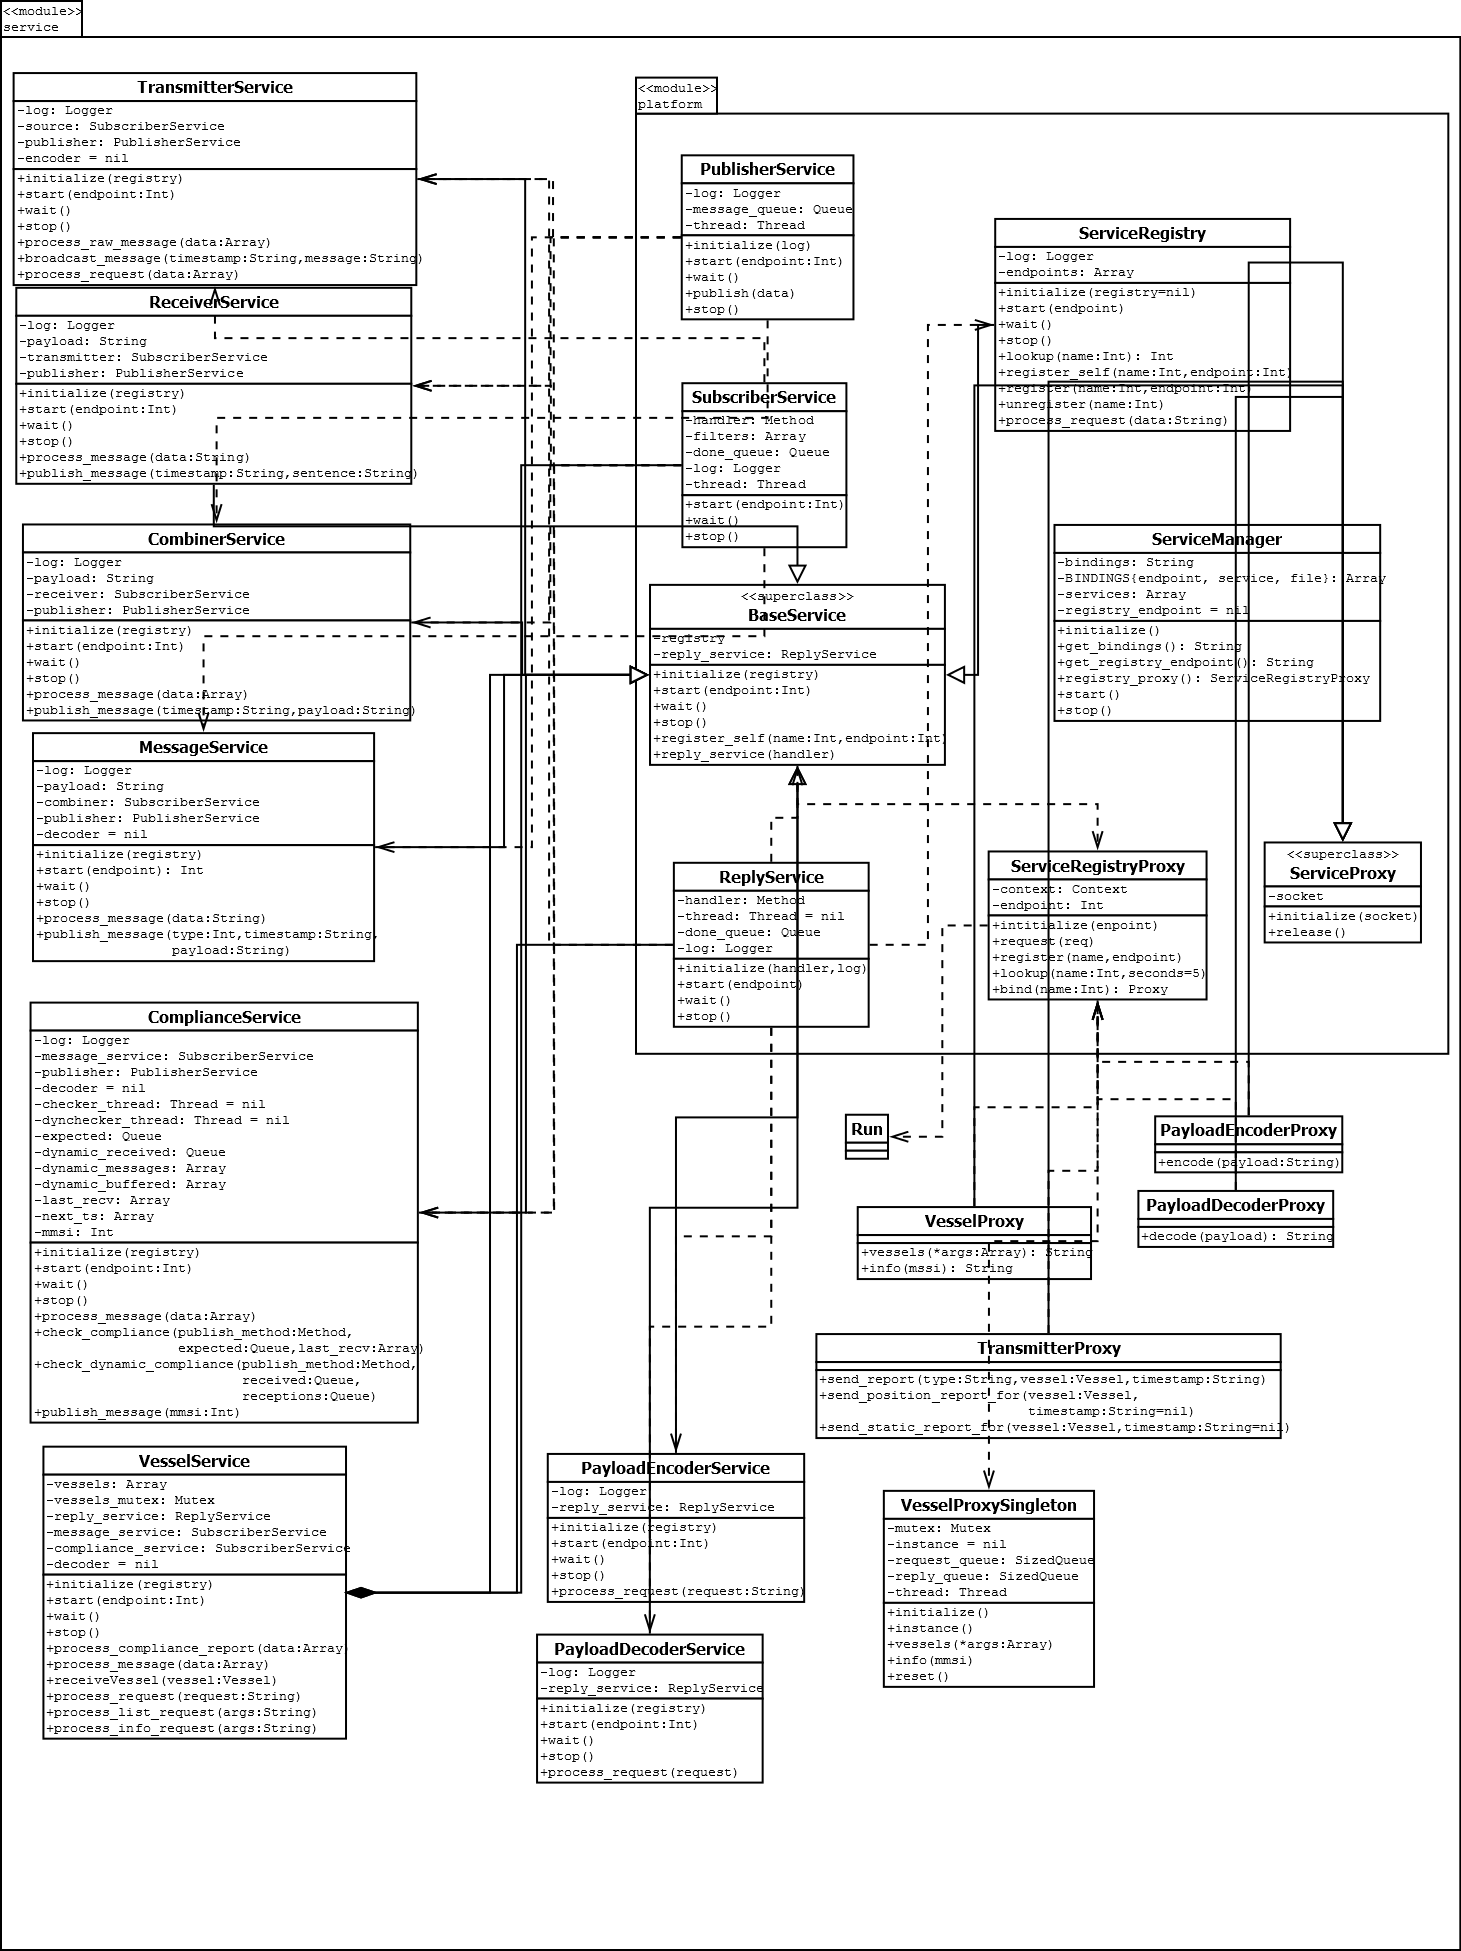
\includegraphics[width=5in]{lib_service_total}
  \caption{A class diagram of the Service module.}
  \label{lib_service_total}
\end{figure}

\begin{figure}
  \centering
  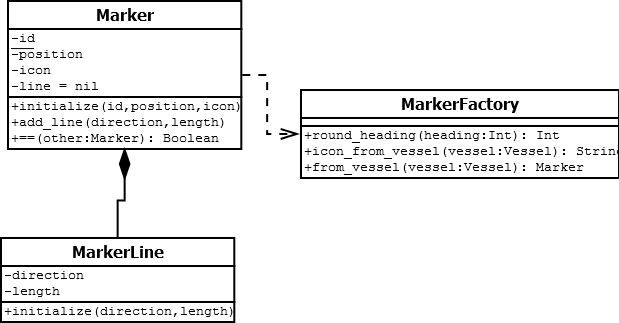
\includegraphics[width=3in]{lib_gis_total}
  \caption{A class diagram of the GIS module.}
  \label{lib_gis_total}
\end{figure}

Visible in the class diagram of the Service module, on the left side of \ref{lib_service_total}, is the pipeline of services, which processes messages from the vessels, starting with TransmitterService and ending with VesselService. This pipeline will be discussed later on, yet in this class diagram the sequence is visible.

\section*{Assignment 2}

\section*{Assignment 3}

\section*{Assignment 4}
For the AIS messages, there is a very strict standard, that all  messages should comply with. From all the messages the system receives, a few do not comply with those standards. This can be due to a lot of things, for example, if the message arrives just a few milliseconds late, the message does not comply. Also, if a vessel moves to fast, regarding the navigational status, the message is deemed non-compliant. To be able to have an idea of how many messages are non-compliant. The system is edited to include a web page, which will show the percentage of compliant messages.

\subsection*{Requirements}
To change in the system has the following requirement
\begin{itemize}
\item There should be a separate web page which will report the percentage of compliant AIS messages received.
\end{itemize}

\subsection*{Realization}
ZO DUS!

\section*{Assignment 5}
The extended AIS program allows a user to view vessels on the map in a range of 65km around the base station. One of the features of this system is to colorize the icons for vessels, so the user can see from the map directly what the type of vessel is. Each color stands for a type of vessel. The program supplied had several colors/vessels implemented, and one of the tasks was to make it possible for the user to recognize more vessels.

\subsection*{Requirements}
The requirements of the change in the system are the following:
\begin{itemize}
\item Vessels of additional different vessel types are to be shown in different colors.
\end{itemize}
\subsection*{Realization}
In the source folder of the project there is a folder with all vessel icons. Every icon has a file name that is built up of several components, with which the icon can be recognised and searched by the program. The build-up of the file name is as follows, and seperated by underscores (\_):
\\
\begin{enumerate}
\item "v" for vessel.
\item "a" of "b" according to the vessel communications device type.
\item Heading, i.e. "n" or "se" according to the given heading.
\item Color: This element makes it possible to couple a color to a vessel.
\item ".png" for the file type.
\end{enumerate}

Finally, the total file with file name "v\_a\_se\_red.png" is taken from the file system. Before this sequence is initiated, the conversion from vessel type to color is done with the following command:
\\
    colors = \{'Passenger' =\textgreater 'green', 'Fishing' =\textgreater 'grey', 'Cargo' =\textgreater 'blue', 'Tanker' =\textgreater 'black', 'Military' =\textgreater 'white', 'Other' =\textgreater 'yellow'\}
\\
\\
From this command, the different colors for different vessel types are gathered. Two boat colors are special and are not generated by this command: red is for vessels that are marked non-compliant by the application and this color is added in a seperate command. Orange is for vessels that are not one of the above vessel types, and this is done by not adding the color tag in the file name.
\\
\\
Now that the system is clear, the new vessel colors can be added. The vessel types that have to be added are: Tug, Towing, Pilot vessel and Port tender. They were given specific colors and the resulting colors can be seen in Table \ref{colortable}.
\\

\begin{table}
\centering

\begin{tabular}{|l|l|}
	\hline
	Passenger & green \\
	\hline
	Fishing & grey \\
	\hline
	Cargo & blue \\
	\hline
	Tanker & black \\
	\hline
	Military & white \\
	\hline
	Other & yellow \\
	\hline
	Tug & brown \\
	\hline
	Towing & beige \\
	\hline
	Pilot vessel & purple \\
	\hline
	Port tender & pink \\
	\hline
	non-compliant & red \\
	\hline
	non of the above & orange \\
	\hline
\end{tabular}
\caption{Table of colors for vessel icons}
\label{colortable}
\end{table}

The resulting command line for the colors is then:
\\
    colors = \{'Passenger' =\textgreater 'green', 'Fishing' =\textgreater 'grey', 'Cargo' =\textgreater 'blue', 'Tanker' =\textgreater 'black', 'Military' =\textgreater 'white', 'Other' =\textgreater 'yellow'\, 'Tug' =\textgreater 'brown', 'Towing' =\textgreater 'beige', 'Pilot vessel' =\textgreater 'purple', 'Port tender' =\textgreater 'pink'\}
\\
\\
After this has been added, the vessel icons were colorized via a photoshop batch process and renamed using windows powershell. They were then placed in the folder with the other vessels.
	


\section*{Assignment 6}
In this system, all messages are fed through a compliance check. This checks if the messages are compliant to the AIS system. In the case that the messages are compliant, nothing is done. But if a message in non-compliant, the vessel that the message originated from will be tagged as non-compliant. The problem with this system is that because the checks are quite strict, and over time almost all the vessels in the system get marked as non-compliant. To solve this, an addition must be made made to the system. After this, when a vessel starts sending compliant messages again, the system sets the state of the vessel back to compliant as the system should have in the first place.

\subsection*{Requirements}
The requirements of the change in the system are the following:
\begin{itemize}
\item Vessels should be marked as non-compliant \emph{if and only when} they send non-compliant AIS messages.
\end{itemize}

\subsection*{Realization}
The changes that where made to the system, in order to meet the requirements are the easiest to see in a sequence diagram. Before the changes, the system was looking like in diagram \ref{diag_compliant_sequence_before}.
\\
TODO: Add awesome sequence diagram before the change.
\\
As can be seen from the diagram, there are a few classes that should be changed.
\begin{itemize}
\item First of all, the ComplianceService should not only report non-compliant messages, but say for every message if the message is compliant or not. This was not too easy, because ComplianceService has two, independent message checking threads. This is fine if you only want to know which vessels are not-compliant, because if one of the two checks fails, that thread publishes the vessel as non-compliant. To fix this, an list of all known vessels is now stored in ComplianceService, and everytime a check passes, it checks in that list if the other check also passed, and then it publishes the vessel as non-compliant. So every time the checks run, they check the last result of the other check for that vessel, so they don't mark vessels as compliant if there not compliant.
\item The second class that needs addition, is the VesselService class. This class must be made compatible with the newly broadcasted messages from ComplianceService and needs to mark vessels compliant again, if CompliantService reports compliant messages. This is a relatively small change.
\end{itemize}

Now, the system works as seen in diagram \ref{diag_compliant_sequence_after}, and meets all the requirements needed.
\\
TODO: Add awesome sequence diagram after the change


\section*{Assignment 7}
Any kind of artefact, especially documents, can be extremely useful to have when working on a software system. The documents should provide \emph{all} information and in addition to the program code, should offer the developer a complete view of the system. This system was delivered with only one document: the installation guide. However very useful for the users who wish to use the system, it offers little information for developers who want to look into the system.

\begin{itemize}
\item System overview\\
A simple document describing how the system is built on a high level. This document should specify the modules that are used to build the system. Also this should show for instance: the user and OpenMaps integration. The goal of this document is to show how different parts are connected (not how they communicate per se) so the developer knows how system design and domain concepts are separated and how the system interacts with other systems.

\item Class diagram\\
A class diagram provides an excellent insight in how the system is actually built. It should be very specific, every attribute and method should be shown, as well as relations between classes. This is very useful to see what the relations between classes are and how they communicate. The class diagram can largely be derived from the code. This makes the class diagram almost a visual implementation of the system.

\item Sequence diagrams and communication diagrams \\
This system can be really tricky when it comes to internal communication. There are a lot of services and it can be very hard to figure out what is happening; what services are used by whom, what is being communicated and how they do that. A sequence diagram can provide this information in very high detail and shows what happens if your system is invoked by for instance a user request or an external message coming in. The latter is the most interesting in our system. A sequence diagram showing what happens when a AIS sentence comes in would have been very useful in understanding this system.

What about communication diagrams? In addition to sequence diagrams, communication diagrams would also have been very useful in understanding how the parts of the system communicate and provide a very good overview of the services. This is something that could be derived from the sequence diagrams, but that can be very tricky. Also, these diagrams can be really helpful when interpreting sequence diagrams. You could compare it to a map and a route description. The Sequence diagram is the route description, telling you how to travel. The map is the overview of all the ways you could travel. Both of these artefacts will bring you to your destination, but the combination makes you fully understand.

\end{itemize}


\section*{Assignment 8}
While reviewing the system, we have come upon three major design faults. First, we'll name the problems and then go into further detail. The first fault we've come across was the fact that there are multiple `MessageX' classes. The second major design fault is the occurrence of implementation details within the domain. The third problem we would like to discuss is the overcomplexity of the decoding pipeline.

\begin{itemize}
\item Multiple `message'-classes\\
The problem with these classes is that they are not in compliance with the 'Single Responsibility Principle'. This specifies that a class should have only one reason to change. Also the 'Liskov Substitution Principle'  is violated. The problem is that there are multiple classes built, while they have almost identical behaviour and properties. The proper way to implement these messages would be to use one superclass 'Message' with an attribute 'message\_type' which is an enum of possible messages. What another option could be is that we crate sub-classes of the superclass `Message'. The superclass holds the data and functions that are the same amongst all messages, while the sub-classes hold individual properties and functions. 
In this particular case, a good design would be to split message types into 2 types: Status update messages and location update messages and make classes for them accordingly. Very important is that a class should only change, when the actual `thing' it models changes, and no other class is affected, but keeping in mind that two different classes that are the same, should be the same class.

\item MessageFactory inside domain\\
After mapping the design of this system it becomes clear that not everything is in the right place. Something is really wrong with the domain part of the system and that is the presence of the class `MessageFactory' within the domain module.

Why is this bad design? 
This is bad because a mix between domain concepts and implementation details has been created. For someone who is new to the system this can be very confusing. The proper way of dealing with this is called `Separation of concerns'. This principle states that the domain model should always be engineered from the actual domain, and not from the system design. What this should accomplish is that the domain model describes the domain concepts, and the system model realizes the system concepts. In general, one must be careful not to mix implementation details with domain concepts and visa versa.

\item Decoding pipeline overcomplexity\\
When looking at the decoding pipeline, we can see that it is pretty long. There are probably two reasons why this is done: First of all, it makes the program more modular and easier to maintain. Secondly, it would allow the maintainer to split the services over multiple machines to spread the workload.

Why is this a bad design?
When designing a system, one must take in to account what tasks it need to accomplish. If this system is only going to be used by one user, does it pay off to have such a long decoding pipeline? In this case it's not. The overhead produced by using a high amount of services has a negative impact on performance, but it has a positive impact on scalability. When scalability is not desired, why use so many services? It increases the complexity of the system, and therefore has a negative impact on maintainability.
\end{itemize}



\end{document}
